% =============================================================================
% Flexible Cable Simulation in NVIDIA Isaac Sim -- progress slides
% Build:  pdflatex cable_slides.tex  (run twice), from this slides/ directory.
% Images come from ../slides_output/{capsule,cosserat_warp,fem}/{cable_only,robot}/frame.png
% (produced by run_all_and_capture.sh); a missing frame shows a labelled placeholder.
% =============================================================================
\documentclass[aspectratio=169]{beamer}
% ===========================================================================
% Theme ported from the master-thesis defense deck (thesis_defense/presentation.tex)
% so this progress deck matches it visually: Madrid + miniframes + circles,
% green/orange scheme, Times fonts.
% ===========================================================================
\usetheme{Madrid}
\setbeamertemplate{navigation symbols}{}
\setbeamertemplate{caption}[numbered]
\usepackage{graphicx}
\usepackage{booktabs}
\usepackage{tikz}

% ---- thesis-defense colour scheme -----------------------------------------
% (names kept from the thesis file; myBlue is actually a green, myTeal an orange)
\definecolor{myBlue}{RGB}{50, 148, 109}
\definecolor{myTeal}{RGB}{229, 61, 0}

\setbeamercolor*{structure}{bg=myBlue,fg=myBlue}
\setbeamercolor*{palette primary}{use=structure,fg=white,bg=structure.fg}
\setbeamercolor*{palette secondary}{use=structure,fg=myBlue,bg=white}
\setbeamercolor*{palette tertiary}{use=structure,fg=white,bg=myBlue}
\setbeamercolor{frametitle}{bg=myBlue,fg=white}
\setbeamercolor*{titlelike}{parent=palette primary}
\setbeamercolor{section in head/foot}{fg=myTeal, bg=white}
\setbeamercolor{item projected}{bg=myTeal}
\setbeamertemplate{enumerate items}{bg=myTeal}
\setbeamercolor{itemize item}{fg=myTeal}
\setbeamercolor{itemize subitem}{fg=myTeal}
\setbeamercolor{button}{bg=myTeal}
\setbeamercolor{section in toc}{fg=black}
\setbeamercolor{subsection in toc}{fg=black}
\setbeamercolor{block title}{bg=myTeal, fg=white}
\setbeamercolor{block body}{bg=myTeal!20}

% ---- fonts (Times, matching the thesis) -----------------------------------
\usefonttheme{professionalfonts}
\usepackage{iftex}
\ifPDFTeX
  \usepackage[T1]{fontenc}
  \usepackage{newtxtext}
  \usepackage{newtxmath}
\else
  \usepackage{fontspec}
  \setmainfont{Times New Roman}
  \setsansfont{Times New Roman}
  \setmonofont{Courier New}
\fi
\usepackage{amsmath}

% ---- extra palette (also from the thesis preamble; used by +/- marks) ------
\colorlet{myred}{red!80!black}
\colorlet{myblue}{blue!80!black}
\colorlet{mygreen}{green!60!black}
\colorlet{mydarkred}{myred!40!black}
\colorlet{mydarkblue}{myblue!40!black}
\colorlet{mydarkgreen}{mygreen!40!black}
\colorlet{myorange}{orange!80!black}
\colorlet{myviolet}{blue!50!red!60}

\useinnertheme{circles}
\useoutertheme{miniframes}
% ---------------------------------------------------------------------------

% This is the SINGLE source .tex; it lives in scripts/cable_simulation/slides/.
% Build it from this directory (run_all_and_capture.sh does this for you):
%   cd scripts/cable_simulation/slides && pdflatex cable_slides.tex   (run twice)
% Frames are referenced as ../slides_output/<method>/<scene>/frame.png (one level up).
\graphicspath{{./}{../}}

% Show a frame.png if it exists, else a neat placeholder box (keeps it compiling).
\newcommand{\simframe}[2]{%   #1 = path, #2 = caption under the image
  \begin{center}
  \IfFileExists{#1}{%
    \includegraphics[height=0.62\textheight,keepaspectratio]{#1}%
  }{%
    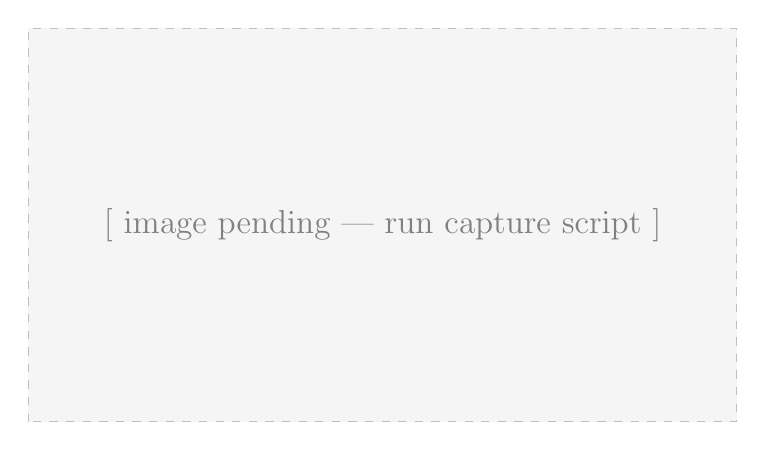
\begin{tikzpicture}
      \draw[gray!50,dashed,fill=gray!8] (0,0) rectangle (9,5.0);
      \node[gray] at (4.5,2.5) {\large [ image pending --- run capture script ]};
    \end{tikzpicture}%
  }\\[2pt]
  {\footnotesize\itshape #2}
  \end{center}}

\title[Cable Simulation in Isaac Sim]{Flexible Cable Simulation in NVIDIA Isaac Sim}
\subtitle{Comparing three modelling approaches for RL-based cable manipulation}
\author[A. Baniasad]{Ali Baniasad}
\institute[U. Waterloo]{Supervisor: Prof.\ Soo Jeon \\ University of Waterloo}
\date{June 2026}

\begin{document}

% ---------- 1. Title ----------
\section{}
\begin{frame}
  \titlepage
\end{frame}

% ---------- Outline ----------
\begin{frame}{Outline}\tableofcontents\end{frame}

\section{Overview}

% ---------- 2. Motivation ----------
\begin{frame}{Motivation}
  \begin{itemize}
    \item \textbf{Why cables?} wire-harness assembly, cable routing, and
          deformable-object manipulation are common, unsolved robotics tasks.
    \item \textbf{The challenge:} Isaac Sim has \emph{no native 1-D deformable
          (rod/cable) body} -- only rigid bodies and volumetric FEM soft bodies.
    \item \textbf{This study:} implement three candidate cable models and lay out
          \emph{what each can and cannot do} -- their capabilities and limitations --
          as a basis for choosing one later for cable manipulation.
  \end{itemize}
  \vfill
  {\footnotesize Three approaches, each in two scenarios (free cable, and cable held
   by a Franka arm). This talk presents trade-offs and limitations -- it does not pick a winner.}
\end{frame}

% ---------- 3. Overview ----------
\begin{frame}{Three approaches}
  \begin{columns}[t]
    \column{0.33\textwidth}\centering
      \textbf{1. Capsule chain}\\\smallskip
      {\footnotesize rigid capsules + D6 joints; bending from Euler--Bernoulli
       beam theory (PhysX).}
    \column{0.33\textwidth}\centering
      \textbf{2. Cosserat rod (Warp)}\\\smallskip
      {\footnotesize 1-D position-based elastic rod in NVIDIA Warp, after the
       \emph{OGC} SIGGRAPH-2025 paper.}
    \column{0.33\textwidth}\centering
      \textbf{3. FEM deformable}\\\smallskip
      {\footnotesize Isaac Sim's built-in volumetric soft body (tetrahedral FEM).}
  \end{columns}
  \vfill
  \begin{center}\footnotesize
  Two scenarios each $\Rightarrow$ \textbf{6 simulations}:
  (A) free hanging/swinging cable \quad (B) cable connected to a robot manipulator.
  \end{center}
\end{frame}

\section{Three approaches}

% ---------- 4. Approach 1 -- cable only ----------
\begin{frame}{Approach 1 --- Capsule chain (D6 joints)}
  \begin{columns}[c]
    \column{0.46\textwidth}
      \begin{itemize}\footnotesize
        \item Rigid capsules linked by \textbf{D6 joints}; translations locked
              (inextensible), bending springs $k=EI/L$ from beam theory.
        \item PhysX \textbf{TGS} solver, up to 200 links, 240\,Hz.
        \item Reproduces the \textbf{Govoni et al.\ 2025} stability sweep [2].
        \item Modes: hanging-kick and both-ends-fixed.
      \end{itemize}
    \column{0.54\textwidth}
      \simframe{../slides_output/capsule/cable_only/frame.png}{Video: 1\_capsule\_cable.mp4 (shared Drive folder)}
  \end{columns}
\end{frame}

% ---------- 5. Approach 1 -- robot ----------
\begin{frame}{Approach 1 --- With robot}
  \simframe{../slides_output/capsule/robot/frame.png}{Video: 1\_capsule\_robot.mp4 (shared Drive folder)}
  \begin{center}\footnotesize
  Inextensible (rigid joints): a hard pull \textbf{drags the second arm $\sim$17\,cm}
  while the cable barely stretches ($\sim$5\,cm) $\Rightarrow$ \textbf{true force transmission}.
  \end{center}
\end{frame}

% ---------- 6. Approach 2 -- cable only ----------
\begin{frame}{Approach 2 --- Cosserat rod in NVIDIA Warp}
  \begin{columns}[c]
    \column{0.46\textwidth}
      \begin{itemize}\footnotesize
        \item 1-D \textbf{Cosserat / XPBD} elastic rod: inextensible stretch +
              bending stiffness + gravity, solved on the GPU in \textbf{Warp}.
        \item Idea from the \textbf{OGC} paper (Chen et al., SIGGRAPH 2025) [1]:
              penetration-free contact for cloth \& rods.
        \item Truly \textbf{thin} (no FEM fattening); \textbf{exact}
              node-vs-primitive collision.
      \end{itemize}
    \column{0.54\textwidth}
      \simframe{../slides_output/cosserat_warp/cable_only/frame.png}{Video: 2\_cosserat\_cable.mp4 (shared Drive folder)}
  \end{columns}
\end{frame}

% ---------- 7. Approach 2 -- robot ----------
\begin{frame}{Approach 2 --- With robot}
  \simframe{../slides_output/cosserat_warp/robot/frame.png}{Video: 2\_cosserat\_robot.mp4 (shared Drive folder)}
  \begin{center}\footnotesize
  End nodes \textbf{pinned} to the grippers: the thin rod follows the arms and sags
  cleanly between them (best-looking cable). \textbf{One-way} -- it follows but exerts
  no force back, so it doesn't drag the second arm.
  \end{center}
\end{frame}

% ---------- 8. Approach 3 -- cable only ----------
\begin{frame}{Approach 3 --- FEM deformable (Isaac Sim)}
  \begin{columns}[c]
    \column{0.46\textwidth}
      \begin{itemize}\footnotesize
        \item Isaac Sim's built-in \textbf{volumetric} (tetrahedral) FEM soft body
              (NVIDIA Omniverse volume-deformable workflow, [3]).
        \item TPU material: $E=40$\,MPa, $\nu=0.48$, $\rho=1150$\,kg/m$^3$.
        \item Rod \textbf{fattened} to 12\,mm and $E$ rescaled so it bends/weighs
              like the real 1.5\,mm cable (voxeliser needs $\geq3$ hexes across).
        \item Rendered thin via a swept tube on its centreline.
      \end{itemize}
    \column{0.54\textwidth}
      \simframe{../slides_output/fem/cable_only/frame.png}{Video: 3\_fem\_cable.mp4 (shared Drive folder)}
  \end{columns}
\end{frame}

% ---------- 9. Approach 3 -- robot ----------
\begin{frame}{Approach 3 --- With robot}
  \simframe{../slides_output/fem/robot/frame.png}{Video: 3\_fem\_robot.mp4 (shared Drive folder)}
  \begin{center}\footnotesize
  Region-weld attachment. Being a soft body it \textbf{stretches a lot} under a hard
  pull ($\sim$20--35\%) and drags the follower little $\Rightarrow$ poor force transmission.
  \end{center}
\end{frame}

\section{Comparison}

% ---------- 10. Trade-offs (neutral, no ranking) ----------
\begin{frame}{Trade-offs at a glance}
  \centering\renewcommand{\arraystretch}{1.25}
  \begin{tabular}{lccc}
    \toprule
    \textbf{Criteria} & \textbf{D6 capsule} & \textbf{Cosserat (Warp)} & \textbf{FEM} \\
    \midrule
    Cable realism       & beam-bending       & 1-D rod (thinnest)      & volumetric (jelly/stretch) \\
    Stretches?          & no (rigid links)   & no (inextensible)       & yes ($\sim$10--50\%) \\
    Thinness            & true 1.5\,mm       & true (any radius)       & $\geq$12\,mm (faked thin) \\
    Compute cost        & low                & low ($\sim$1.4$\times$ RT) & high ($<$0.2$\times$ RT) \\
    Robot force coupling& two-way            & one-way (or spring)     & two-way (rough) \\
    Collision           & exact capsules     & exact (coded prims)     & approximate tets \\
    Setup / code        & many joints        & custom Warp solver      & built-in \\
    \bottomrule
  \end{tabular}
  \vfill
  {\footnotesize RT = real time. These are \emph{trade-offs} -- no single method wins
   on every row; the right one depends on the priority.}
\end{frame}

% ---------- 11. Pros & cons (no ranking) ----------
\begin{frame}{Pros and cons (each is a trade-off --- no single ``best'')}
  \footnotesize
  \textbf{1. Capsule chain (D6 joints)}
  \begin{itemize}\itemsep0pt
    \item[\textcolor{mygreen}{+}] Stable; physically grounded; real-time; two-way force coupling; easy to randomize.
    \item[\textcolor{myred}{--}] Piecewise-rigid (no axial give); many bodies; needs a heavy solver to stay inextensible.
  \end{itemize}
  \textbf{2. Cosserat rod in Warp (OGC)}
  \begin{itemize}\itemsep0pt
    \item[\textcolor{mygreen}{+}] Thinnest, cleanest cable; inextensible; no jelly; exact node-vs-primitive collision; GPU-fast.
    \item[\textcolor{myred}{--}] Separate (non-PhysX) sim; only artificial robot coupling; hand-coded collision; custom solver.
  \end{itemize}
  \textbf{3. FEM deformable}
  \begin{itemize}\itemsep0pt
    \item[\textcolor{mygreen}{+}] True volumetric soft body; native to Isaac Sim; two-way; handles squashing/draping.
    \item[\textcolor{myred}{--}] Fat, stretches, jelly, rigid at the joint, rough collision, slow.
  \end{itemize}
\end{frame}

\section{Limitations}

% ---------- 12. Limitations: Capsule ----------
\begin{frame}{Limitations --- Capsule chain (D6 joints)}
  \footnotesize
  \begin{itemize}\itemsep2pt
    \item \textbf{Piecewise-rigid:} links cannot stretch \emph{at all} -- it is a chain
          of rigid bodies, not a continuum; bending is a discrete per-joint spring.
    \item \textbf{Many bodies:} needs 60--200 links + joints for a smooth look
          $\Rightarrow$ many rigid bodies and constraints to simulate.
    \item \textbf{Solver cost vs.\ rigidity:} staying inextensible under load needs
          high position-iteration counts ($\approx$180); too few $\Rightarrow$ it
          stretches, too many $\Rightarrow$ it goes unstable.
    \item \textbf{Numerical twist:} the free twist DOF spins up unless explicitly damped.
    \item \textbf{Tuning-sensitive:} link mass / joint stiffness / damping / timestep
          must be balanced (mass-ratio \& dt limits) or the chain diverges.
    \item \textbf{Approximate bending:} torsional springs from beam theory, not a true rod.
  \end{itemize}
\end{frame}

% ---------- 13. Limitations: Warp rod ----------
\begin{frame}{Limitations --- Cosserat rod (Warp / OGC)}
  \footnotesize
  \begin{itemize}\itemsep2pt
    \item \textbf{Not a native physics body:} it is a \emph{separate} Warp simulation
          $\Rightarrow$ it does not interact with PhysX bodies through the engine
          (no automatic contact with robots or objects).
    \item \textbf{Artificial robot coupling:} either kinematic (\textbf{one-way} --
          follows the gripper, no force back) or a hand-tuned spring (two-way, but then
          it visibly \emph{stretches}); no clean physical two-way coupling.
    \item \textbf{Hand-coded collision only:} node-vs-primitive (ground, sphere) that
          you write; no general mesh contact, no self-collision unless coded.
    \item \textbf{Implementation burden:} you must write \& maintain the XPBD solver
          kernels -- not off-the-shelf; every new obstacle needs custom contact code.
  \end{itemize}
\end{frame}

% ---------- 14. Limitations: FEM ----------
\begin{frame}{Limitations --- FEM deformable}
  \footnotesize
  \begin{itemize}\itemsep1pt
    \item \textbf{Cannot be thin:} voxeliser needs $\geq$3 hexes across the diameter and
          cooking caps resolution $\Rightarrow$ thinnest $\approx$12\,mm (real cable
          1.5\,mm, $8\times$ too thick); only \emph{rendered} thin.
    \item \textbf{Stretches:} one isotropic $E$ ties bending ($\propto E r^4$) to axial
          ($\propto E r^2$) -- exact bending $\Rightarrow$ axially soft ($\sim$50\%
          stretch); firm enough not to stretch $\Rightarrow$ bending 20--30$\times$ too stiff.
    \item \textbf{``Jelly'':} low-resolution soft body + near-incompressible $\nu$
          $\Rightarrow$ volumetric locking / wobble.
    \item \textbf{Rigid at the connection:} attachment \emph{welds a region} of vertices
          (clamped-beam boundary) $\Rightarrow$ straight/stiff near the joint, not a pin.
    \item \textbf{Rough collision:} simplified, re-meshed coarse collision tets
          $\Rightarrow$ imprecise, can clip thin obstacles; self-collision off by default.
    \item \textbf{Expensive:} GPU FEM runs $<$0.2$\times$ real-time.
  \end{itemize}
\end{frame}

\section{References}

% ---------- 15. References ----------
\begin{frame}{References}
  \footnotesize
  \begin{itemize}\itemsep4pt
    \item[{[1]}] A. H. Chen, J. Hsu, Z. Liu, M. Macklin, Y. Yang, and C. Yuksel.
          \textbf{Offset Geometric Contact.}
          \emph{ACM Transactions on Graphics} (SIGGRAPH 2025), 44(4), 2025.
          DOI: 10.1145/3731205. \\
          {\scriptsize Source for Approach~2 (Cosserat / position-based rod in NVIDIA Warp).
           \texttt{graphics.cs.utah.edu/research/projects/ogc}}
    \item[{[2]}] A. Govoni, N. Zubair, S. Soprani, and G. Palli.
          \textbf{Performance Analysis of a Mass--Spring--Damper Deformable Linear
          Object Model in Robotic Simulation Frameworks.}
          European Robotics Forum (ERF), 2025. arXiv:2504.13659. \\
          {\scriptsize Reference for the Approach~1 DLO / stability behaviour.}
    \item[{[3]}] NVIDIA. \textbf{Omniverse Physics Extension --- Volume Deformables (Overview).}
          Omniverse tutorial video. \texttt{youtube.com/watch?v=focL232tb8U} \\
          {\scriptsize Source for Approach~3 (Isaac Sim volumetric FEM soft body).}
  \end{itemize}
\end{frame}

% ---------- 16. Thanks ----------
\begin{frame}[plain]
  \centering\vfill
  {\Large Thank you}\\[3em]
  {\footnotesize Ali Baniasad --- Supervisor: Prof.\ Soo Jeon, University of Waterloo}
  \vfill
\end{frame}

\end{document}
